%% arara directives
% arara: xelatex
% arara: bibtex
% arara: xelatex
% arara: xelatex

%\documentclass{article} % One-column default
\documentclass[twocolumn, switch]{article} % Method A for two-column formatting

\usepackage{preprint}

%% Math packages
\usepackage{amsmath, amsthm, amssymb, amsfonts}

%% Bibliography options
\usepackage[numbers,square]{natbib}
\bibliographystyle{unsrtnat}
%\usepackage{natbib}
%\bibliographystyle{Geology}

%% General packages
\usepackage[utf8]{inputenc}	% allow utf-8 input
\usepackage[T1]{fontenc}	% use 8-bit T1 fonts
\usepackage{booktabs} 		% professional-quality tables
\usepackage{nicefrac}		% compact symbols for 1/2, etc.
\usepackage{microtype}		% microtypography
\usepackage{lineno}		% Line numbers
\usepackage{float}			% Allows for figures within multicol
%\usepackage{multicol}		% Multiple columns (Method B)

% \usepackage{lipsum}		%  Filler text
\usepackage{listings}   % Code formatter

\graphicspath{{images/}}
% \pagenumbering{arabic}

\lstset{
  basicstyle=\ttfamily,
  columns=fullflexible,
  breaklines=true,
  postbreak=\raisebox{0ex}[0ex][0ex]{\color{red}$\hookrightarrow$\space}
}

 %% Special figure caption options
\usepackage{newfloat}
\DeclareFloatingEnvironment[name={Supplementary Figure}]{suppfigure}
\usepackage{sidecap}
\sidecaptionvpos{figure}{c}

% Section title spacing  options
\usepackage{titlesec}
\titlespacing\section{0pt}{12pt plus 3pt minus 3pt}{1pt plus 1pt minus 1pt}
\titlespacing\subsection{0pt}{10pt plus 3pt minus 3pt}{1pt plus 1pt minus 1pt}
\titlespacing\subsubsection{0pt}{8pt plus 3pt minus 3pt}{1pt plus 1pt minus 1pt}

% ORCiD insertion
\usepackage{tikz, xcolor, hyperref}
% \usepackage[[pdftex, pdfauthor={Jovial Joe Jayarson}, pdftitle={Vudoku - Visual Sudoku Solver}, pdfsubject={Digit Recognition, Computer Vision}]{hyperref}

\hypersetup{
  colorlinks      = true,
  urlcolor        = gray,
  linkcolor       = magenta,
  citecolor       = brown,
  citebordercolor = green,
  urlbordercolor  = white,
  linkbordercolor = blue,
}

\definecolor{lime}{HTML}{A6CE39}
\DeclareRobustCommand{\orcidicon}{
	
\begin{tikzpicture}
	\draw[lime, fill=lime] (0,0) 
	circle [radius=0.16] 
	node[white] {{\fontfamily{qag}\selectfont \tiny ID}};
	\draw[white, fill=white] (-0.0625,0.095) 
	circle [radius=0.007];
	\end{tikzpicture}
	\hspace{-2mm}
}
\foreach \x in {A, ..., Z}{\expandafter\xdef\csname orcid\x\endcsname{\noexpand\href{https://orcid.org/\csname orcidauthor\x\endcsname}
			{\noexpand\orcidicon}}
}
% Define the ORCID iD command for each author separately. Here done for two authors.
\newcommand{\orcidauthorA}{0000-0001-7002-9923}
\newcommand{\orcidauthorB}{0000-0001-8302-796X}
% \newcommand{\orcidauthorC}{0000-0000-0000-0003}
% \newcommand{\orcidauthorD}{0000-0000-0000-0004}

%%%%%%%%%%%%%%%%   Title   %%%%%%%%%%%%%%%%
\title{Vudoku - A Visual Sudoku Solver}

% Add watermark with submission status
\usepackage{xwatermark}
% Left watermark
\newwatermark[firstpage,color=gray!60,angle=90,scale=0.32, xpos=-3.9in,ypos=0]{\href{https://doi.org/}{\color{gray}{Publication DOI}}}
% Right watermark
\newwatermark[firstpage,color=gray!60,angle=90,scale=0.32, xpos=3.8in,ypos=0]{\href{https://doi.org/}{\color{gray}{Preprint DOI}}}
% Bottom watermark
\newwatermark[firstpage,color=gray!90,angle=0,scale=0.28, xpos=0in,ypos=-5in]{*correspondence: \texttt{jovial7joe@hotmail.com}}

%%%%%%%%%%%%%%%  Author list  %%%%%%%%%%%%%%%
\usepackage{authblk}
\renewcommand*{\Authfont}{\bfseries}
\author[+\thanks{\tt{jovial7joe@hotmail.com}}]{Jovial Joe Jayarson\orcidA{}}
\author[+]{Ebin P M\orcidB{}}

\affil[+]{Department of Computer Science \& Engineering, IESCE}
\affil[+]{APJ Kalam Technological University}

% Option 2 for author list
%\author{
%  David S.~Hippocampus\thanks{Use footnote for providing further
%    information about author (webpage, alternative
%    address)---\emph{not} for acknowledging funding agencies.} \\
%  Department of Computer Science\\
%  Cranberry-Lemon University\\
%  Pittsburgh, PA 15213 \\
%  \texttt{hippo@cs.cranberry-lemon.edu} \\
%  %% examples of more authors
%   \And
% Elias D.~Striatum \\
%  Department of Electrical Engineering\\
%  Mount-Sheikh University\\
%  Santa Narimana, Levand \\
%  \texttt{stariate@ee.mount-sheikh.edu} \\
%  \AND
%  Coauthor \\
%  Affiliation \\
%  Address \\
%  \texttt{email} \\
%  % etc.
%}

%%%%%%%%%%%%%%    Front matter    %%%%%%%%%%%%%%
\begin{document}

\twocolumn[ % Method A for two-column formatting
  \begin{@twocolumnfalse} % Method A for two-column formatting

    \maketitle

    \begin{abstract}
      It is no secret that AI is an upcoming titan. Even though people are stunned to hear that AI has been here for around a century, due to the advancement in computational methods and resources, today AI peaks like never before. As a tiny glimpse into the field of Digit Recognition, this project aims to understand the underlying cogs and wheels on which the neural networks spin. This paper tries to elucidate a project which solves the Sudoku puzzle drawn and written by hand. The paraphernalia for that project includes programming language: Python3; libraries: OpenCV, Numpy, Keras/Tensorflow; datasets: MNIST handwritten digit database.  Digit recognition is a classical problem which will introduce neurons, neural networks, connections hidden layers, weights, biases, activation functions like sigmoid, back-propagation and other related topics as well. Algorithm(s) in the project employed to solve Sudoku is also explored in this paper.
    \end{abstract}
    \keywords{Machine Learning \and Artificial Intelligence \and Computer Vision \and Sudoku Puzzle \and Neural Networks \and Back Tracking}
    \vspace{0.35cm}

  \end{@twocolumnfalse} % Method A for two-column formatting
] % Method A for two-column formatting

%\begin{multicols}{2} % Method B for two-column formatting (doesn't play well with line numbers), comment out if using method A


%%%%%%%%%%%%%%%  Main text   %%%%%%%%%%%%%%%
% \linenumbers

\section{Introduction}
\label{sec:introduction}
Machines are inherently incapable to understand, text, images and audio. These formats which carry information, needs to be converted into numbers, matrices or vectors which is a significant step, in any procedure, to solve problems using computers. Another vital stage for digit recognition is \emph{machine learning}. With classical problem solving techniques, humans provide computers with both data and rules as input. In contrast, we provides data and presumed result, as input to a machine learning system. And then we let it find out some \emph{rules}. A quick example would be to give three numbers $x$, $y$ and $z$ and tell a machine that - certain operation was performed on $x$ and $y$ to obtain $z$. Once a machine is fed with lots and lots of similar examples, it will be equipped find out some pattern behind it. At a later stage, it can very well predict, what operations might have been performed on $x$ and $y$ to result in $z$. Sudoku is a mathematical problem and by default has $9\times 9$ grids. There are other variant to it but to keep things simple, the project moves along with the default one. Sudoku is classified as Exact Cover or Hitting Set problem \cite{wiki:exactcover}. Various algorithms has been developed over the years to solve it, like Backtracking, Stochastic algorithms, Constraint programming and so on. Given that the output of the digit recognition system is as \emph{value}, \emph{position} pairs or and \emph{encoded string}, this project uses simple backtracking algorithm to solve Sudoku.


\section{Contemporary Technologies}
\label{sec:contemporaryTech}
Complex problems exists all around us. Some of them are stumbled upon and other have be thoughtfully crafted. Solutions to these problems at times are intuitive and yet difficult to explain. Structured mathematical approach to problems has engineered some of the finest solutions to some of the toughest problem. In the era of computing, appetite to solve problems using machines has become a hobby. With technology at fingertips, it's no-brainer that upcoming generations have a choice to be way smarter. It's of no surprise that the field of artificial intelligence has come a long way. This section deals with some of the famous models and how they are related to digit recognition. Starting from the ones released in 80's like \emph{Recurrent Neural Network (RNN)} to the latest 2017 model \emph{The Transformer}, much study has been conducted.

\subsection{Recurrent Neural Network}
\label{sub:sec:rnn}
Basic RNNs are a network of neuron-like nodes organized into successive layers. Each node in a given layer is connected with a directed (one-way) connection to every other node in the next successive layer. The following figure \eqref{fig:2.1} gives the internal schematics of Recurrent Neural Networks.

\begin{figure}[!htbp]
    \centering
    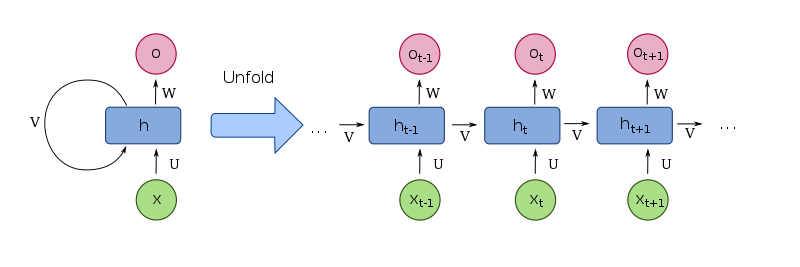
\includegraphics[width=0.5\textwidth]{Recurrent_neural_network_unfold.png}
    \caption[Recurrent Neural Networks Unfolded]{Recurrent Neural Networks Unfolded \cite{wiki:rnns}}
    \label{fig:2.1}
\end{figure}

Each node (neuron) has a time-varying real-valued activation. Each connection (synapse) has a modifiable real-valued weight. Nodes are either input nodes (receiving data from outside of the network), output nodes (yielding results), or hidden nodes (that modify the data en route from input to output). Each sequence produces an error as the sum of the deviations of all target signals from the corresponding activations computed by the network. For a training set of numerous sequences, the total error is the sum of the errors of all individual sequences. The following equation \eqref{equ:2.1} was proposed as part of research on \emph{Simple Recurrent Neural Network} \cite{wiki:rnns}:

\[h_t = \sigma_h(W_h x_t + U_h y_{t-1} + b_h)\]
\begin{equation}
    \label{equ:2.1}
    y_t = \sigma_y(W_y h_t + b_y)
\end{equation}

Where, $x_t$ is input vector, $h_t$ is hidden layer vector, $y_t$ is output vector, $W, U$ and $b$ are parameter matrices and vector, respectively $\sigma_h$ and $\sigma_y$ are activation functions.

Recurrent neural networks models contain a self-connected hidden layer. One benefit of the recurrent connection is that a `memory' of previous inputs remains in the network’s internal state, allowing it to make use of past context. This is significant for handwriting recognition as mentioned in \cite{art:ieee:consys}. A major problem with gradient descent for standard RNN architectures is that error gradients vanish exponentially quickly with the size of the time lag between important events \cite{wiki:rnns}.

\subsection{Long Short Term Memory}
\label{sub:sec:lstm}

Long short-term memory (LSTM) is a deep learning system that avoids the vanishing gradient problem. LSTM is normally augmented by recurrent gates called ``forget gates''. LSTM prevents backpropagated errors from vanishing or exploding. Instead, errors can flow backwards through unlimited numbers of virtual layers unfolded in space. That is, LSTM can learn tasks that require memories of events that happened thousands or even millions of discrete time steps earlier \cite{wiki:rnns}.

\begin{figure}[!htbp]
    \centering
    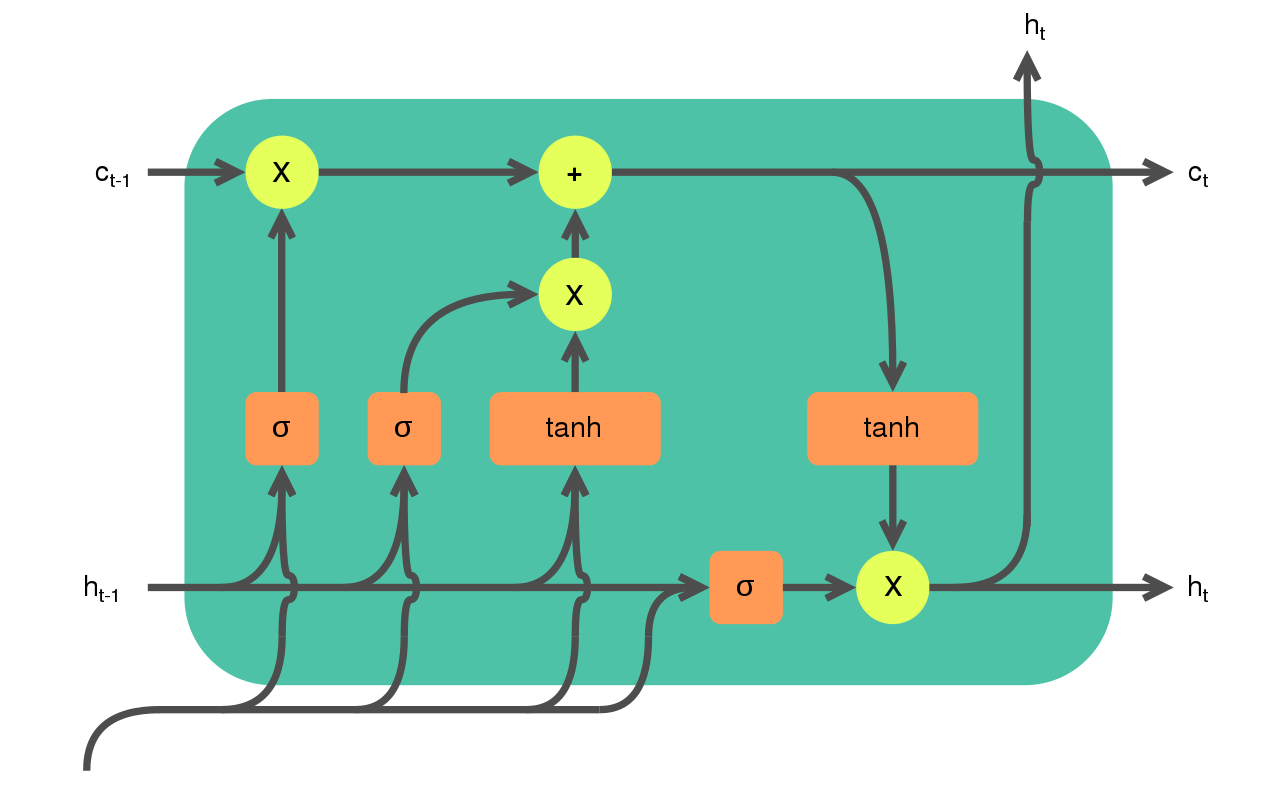
\includegraphics[width=0.4\textwidth]{LSTM_cell.png}
    \caption[Long Short Term Memory Cell]{Long Short Term Memory Cell \cite{wiki:lstm}}
    \label{fig:2.2}
\end{figure}

A common LSTM unit, as shown in figure \eqref{fig:2.2}, is composed of a cell, an \emph{input gate}, an \emph{output gate} and a \emph{forget gate}. The cell remembers values over arbitrary time intervals and the three gates regulate the flow of information into and out of the cell. Some variations of the LSTM unit do not have one or more of these gates or maybe have other gates. For example, \emph{Gated Recurrent Units} (GRUs) do not have an output gate. LSTM networks are hence well-suited for classifying time series data.

\subsection{Convolutional Neural Networks}
\label{sub:sec:cnnlr}

A convolutional neural network (CNN), is a class of deep neural networks, most commonly applied to analyzing visual imagery. They are also known as shift invariant or \emph{space invariant artificial neural networks} (SIANN). CNNs have a wide variety of applications including, image and video recognition, recommender system, brain-computer interface etc. CNNs are regularized versions of multilayer perceptrons. Multilayer perceptrons usually mean fully connected networks, that is, each neuron in one layer is connected to all neurons in the next layer.

Convolutional networks were inspired by biological processes in that the connectivity pattern between neurons resembles the organization of the animal visual cortex. CNNs use relatively less pre-processing compared to other image classification algorithms. Independence from prior knowledge and human effort in feature design is a major advantage \cite{wiki:cnns}


\section{Project Walk-through}
\label{sec:projectwkt}
The goal of the project as stated in the abstract and introduction section \eqref{sec:introduction}, is to solve a Sudoku puzzle which is provided as an visual input to the computer. Being a multidisciplinary problem, it contains various modules laid out neatly. Below is the directory structure of the project: 

\begin{lstlisting}
|-- src/
    |-- samples/
    |-- classifier.py
    |-- extractor.py
    |-- main.py
    |-- scavenger.py
    |-- solver.py
|-- README.md
|-- LICENSE
\end{lstlisting}

As obvious the \lstinline{main.py} script plays the pivotal role of managing the control flow. It's a \href{https://github.com/streamlit/streamlit/}{Streamlit} application. The UI layer looks like as shown in figure \eqref{fig:3.1} and \eqref{fig:3.2}.

\begin{figure}[!htbp]
    \centering
    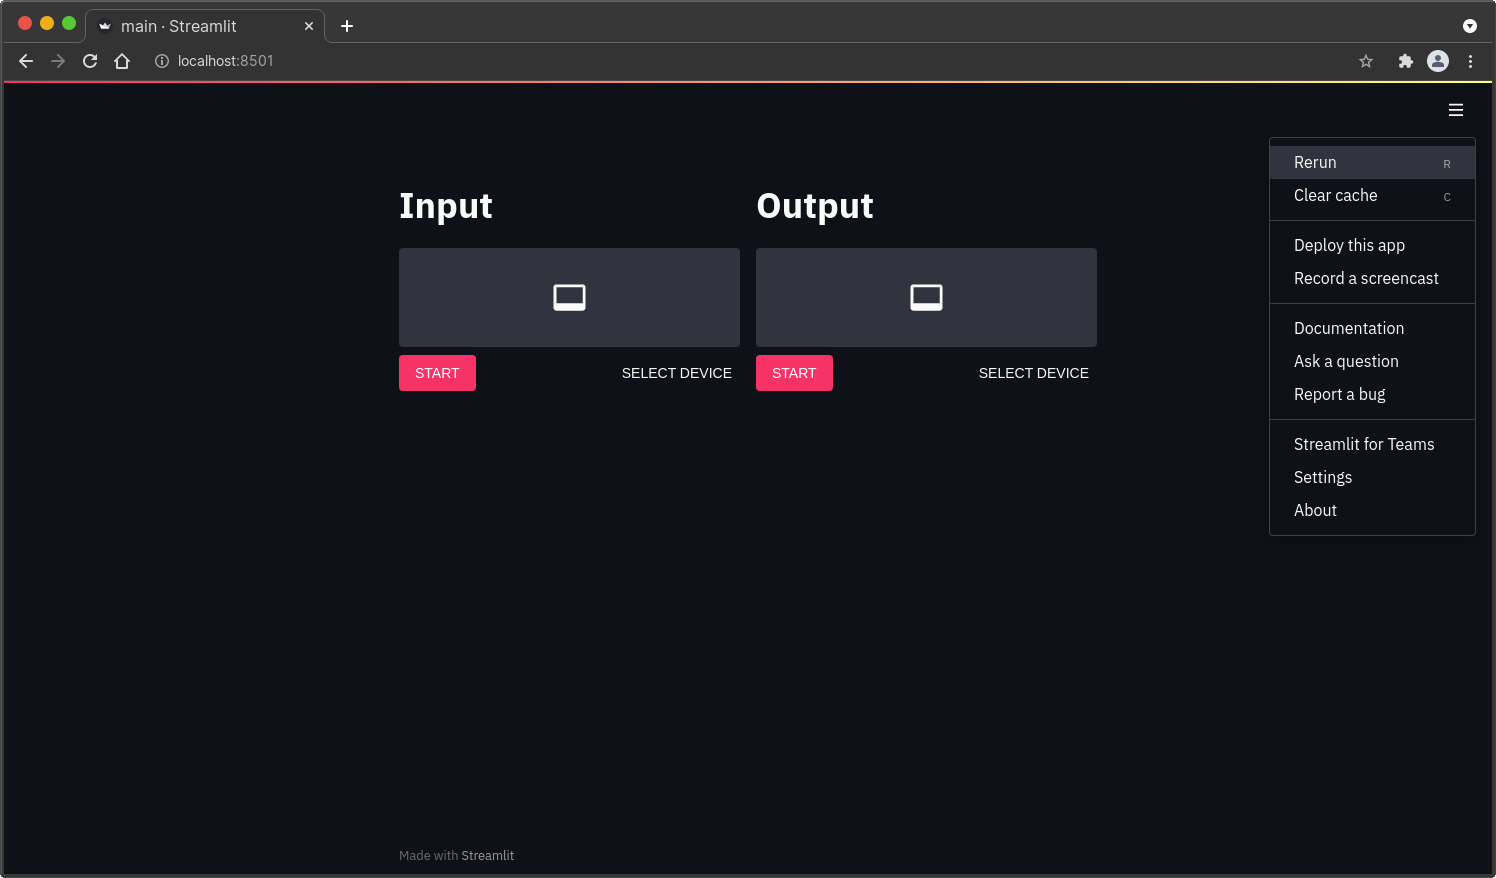
\includegraphics[width=0.3\textwidth]{wireframe_ui.png}
    \caption[Vudoku UI]{\centering Vudoku UI}
    \label{fig:3.1}
\end{figure}

\begin{figure}[!htbp]
    \centering
    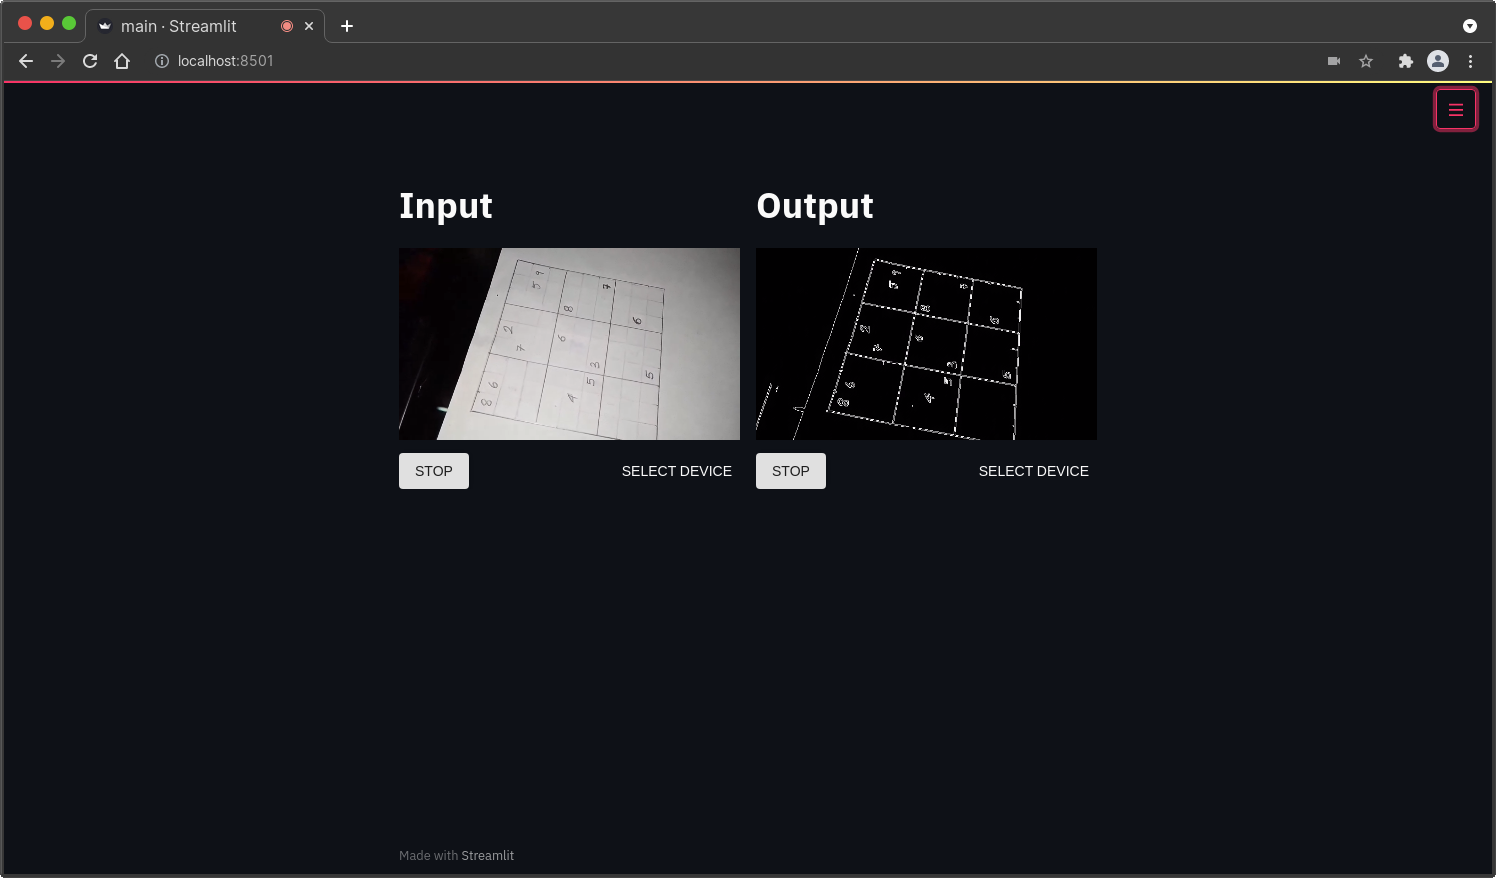
\includegraphics[width=0.3\textwidth]{processing.png}
    \caption[Edge Detection]{\centering Edge Detection}
    \label{fig:3.2}
\end{figure}

\subsection{Scavenger}
\label{sub:sec:scavenger}
This module is what takes the input and in human terms tries to understand it. It expects a similar input, where Sudoku is prominent in the input image as shown in \eqref{fig:3.1}.

\begin{figure}[!htbp]
    \centering
    \begin{minipage}{0.24\textwidth}
        \centering
        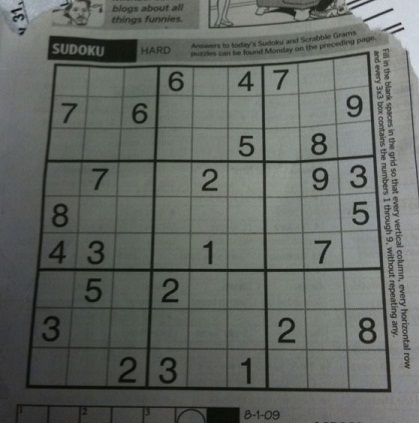
\includegraphics[height=0.5\textwidth]{sample_puzzle.jpg}
        \caption[Sample Input]{\centering Sample Input}
        \label{fig:3.3}
    \end{minipage}\hfill
    \begin{minipage}{0.24\textwidth}
        \centering
        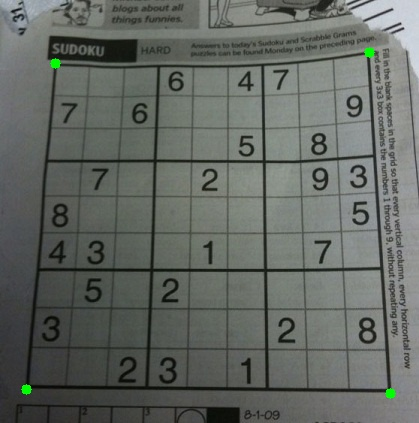
\includegraphics[height=0.5\textwidth]{corners.jpg}
        \caption[Sample Input]{\centering Contours Points}
        \label{fig:3.4}
    \end{minipage}
\end{figure}

It finds contours points that encapsulate the maximum area which is shown in \eqref{fig:3.2}. Finally performs a perspective transform that takes to contours points, extracts that area and superimposes it on a blank image to obtain the resultant image as in \eqref{fig:3.3}

\begin{figure}[!htbp]
    \centering
    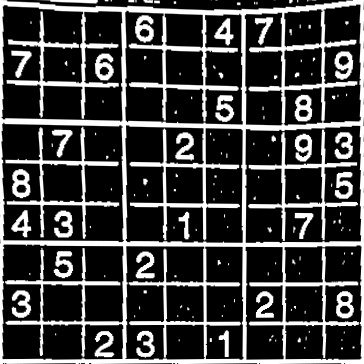
\includegraphics[width=0.3\textwidth]{transformed.jpg}
    \caption[Transformed Sudoku]{Transformed Sudoku}
    \label{fig:3.5}
\end{figure}

\subsection{Extractor}
\label{sub:sec:extractor}
The extractor module grabs each cell from the transformed Sudoku board and arranges them in a list. Then it loads a classifier \eqref{sub:sec:classifier} and classifies the image data in the cell into a number. Each of these number are string concatenated to obtain a 81 bit long string after the process.

\subsection{Solver}
\label{sub:sec:solver}
Solver is an implementation of backtracking algorithm employed to solve Sudoku in specific. It verifies uniqueness in each row column and sub box while recursively filling out the puzzle. Finally it spits out an 81 bit long solution string. This string can be later manipulated to one's liking.

\subsection{Classifier}
\label{sub:sec:classifier}
The digit classifier module does not actively participate in the control flow, the reason being the existence of a saved model. If need arises for a more granular control, then a new model must be generate tuning the hyper-parameters. Speaking of which this model is a sandwich of

\lstinline{2D Convolution Network with ReLu activation + another 2D Convolution Network with ReLu activation  + a 2D Max-Pooling layer + Flattened Layer + Dense Network with ReLu activation + Dense Network with SoftMax activation}

The CNN architecture is best depicted by figure \eqref{fig:3.6}

\begin{figure}[!htbp]
    \centering
    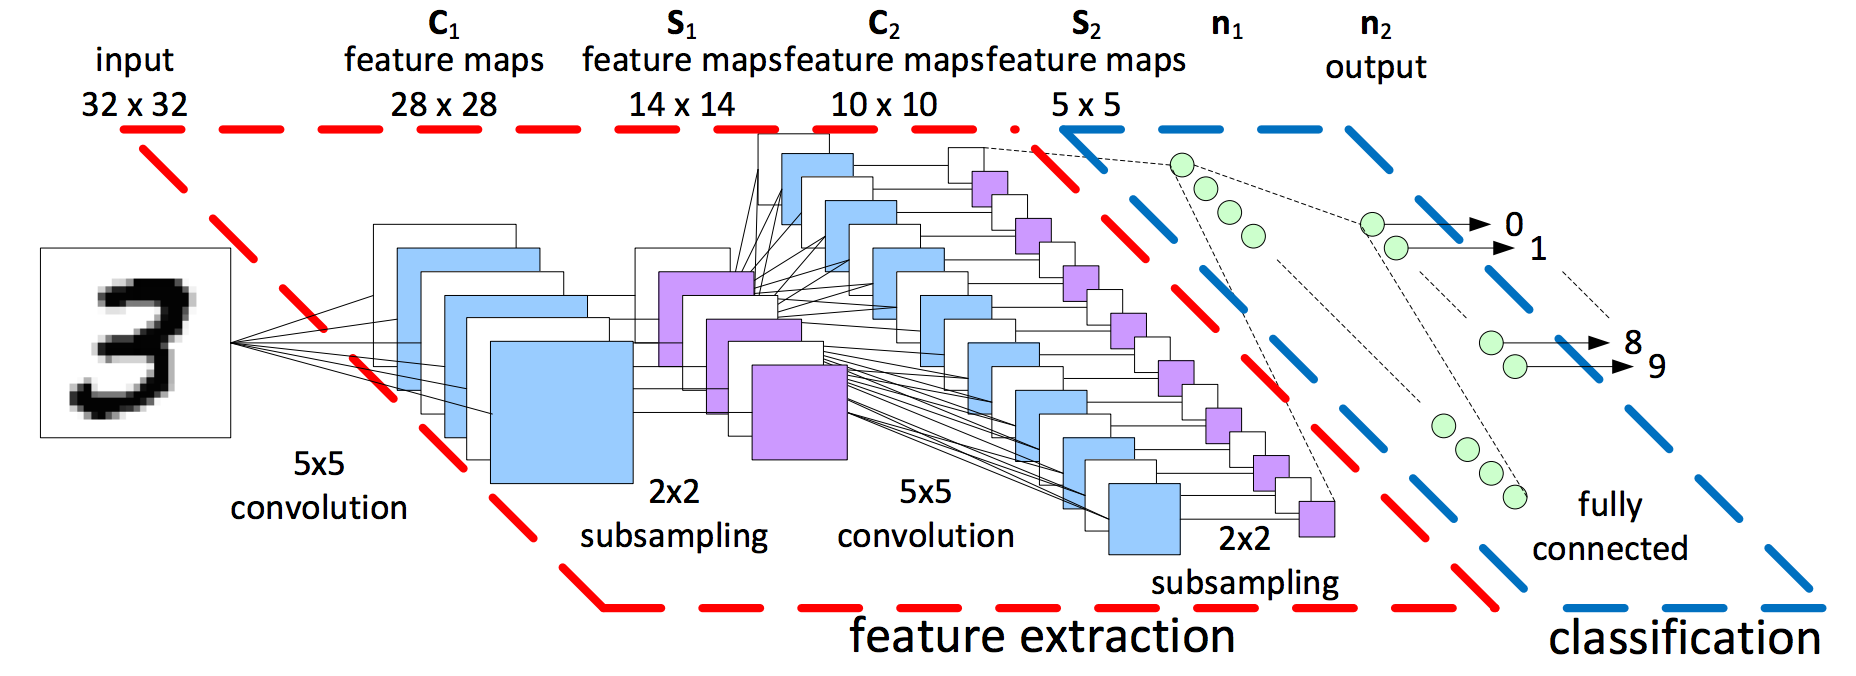
\includegraphics[width=0.4\textwidth]{cnn_layers.png}
    \caption[Digit cells]{Digit cells}
    \label{fig:3.6}
\end{figure}

\section{Conclusion}
\label{sec:conclusion}
Digit recognition is an interesting classical problem to embark the journey in the field of artificial intelligence. Sudoku, a mathematical puzzle is captivating beauty of the mystery that lies in various patterns and combinations in itself. Visualizing Sudoku will give an insight on many aspects, including accuracy, performance, complexity, precision, recall etc. This project could be an inspiring stepping stone for futures enthusiasts to work upon.

%%%%%%%%%%%% Supplementary Methods %%%%%%%%%%%%
%\footnotesize
%\section*{Methods}

%%%%%%%%%%%%% Acknowledgements %%%%%%%%%%%%%
%\footnotesize
%\section*{Acknowledgements}

%%%%%%%%%%%%%%   Bibliography   %%%%%%%%%%%%%%
\normalsize
\bibliography{references}

%%%%%%%%%%%%  Supplementary Figures  %%%%%%%%%%%%
%\clearpage

%%%%%%%%%%%%%%%%   End   %%%%%%%%%%%%%%%%
%\end{multicols}  % Method B for two-column formatting (doesn't play well with line numbers), comment out if using method A
\end{document}
